\documentclass{standalone}
\usepackage[usenames,dvipsnames]{xcolor}
\usepackage{tikz}
\usepackage[utf8]{inputenc}
\usepackage[T1]{fontenc}
\usepackage[upright]{fourier}
%\usepackage[dvipsnames]{xcolor}
\usepackage{tkz-kiviat,numprint,fullpage}
\usepackage{capt-of}
\usepackage{pgfplots}
\usetikzlibrary{arrows}
%\usepackage[dvipsnames]{xcolor}
\input{USAmap.tex}
%\newcommand{\cbox}[2]{\raisebox{\depth}{\fcolorbox{black}{#1}{\null}}}
\begin{document}

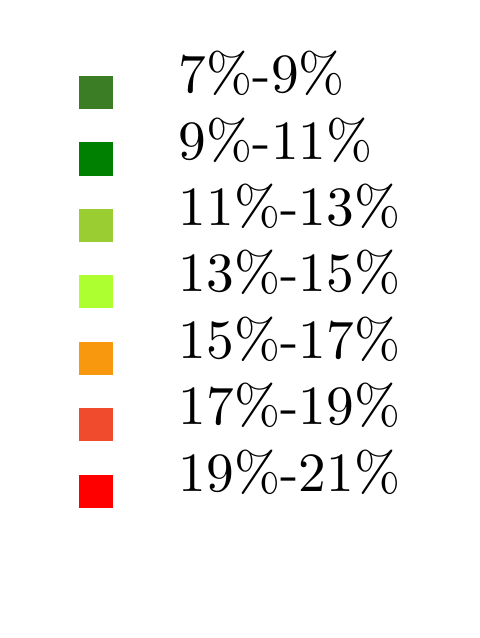
\begin{tikzpicture}


%\tikzset{set state val/.style args={#1/#2}{#1={fill=blue!#2}}}
%\tikzset{set state val/.list={CA/100,FL/80,TX/55,NY/20}}

\USA[every state={draw=white, ultra thick, fill=black!10},AL ={fill= YellowOrange }, AK ={fill= YellowGreen }, AZ ={fill= GreenYellow }, AR ={fill= RedOrange }, CA ={fill= GreenYellow }, CO ={fill= YellowGreen }, CT ={fill= OliveGreen }, DE ={fill= Green }, DC ={fill= Red }, FL ={fill= YellowGreen }, GA ={fill= GreenYellow }, HI ={fill= Green }, ID ={fill= GreenYellow }, IL ={fill= YellowGreen }, IN ={fill= YellowGreen }, IA ={fill= Green }, KS ={fill= YellowGreen }, KY ={fill= YellowOrange }, LA ={fill= Red }, ME ={fill= YellowGreen }, MD ={fill= OliveGreen }, MA ={fill= Green }, MI ={fill= GreenYellow }, MN ={fill= Green }, MS ={fill= Red }, MO ={fill= GreenYellow }, MT ={fill= GreenYellow }, NE ={fill= Green }, NV ={fill= YellowGreen }, NH ={fill= OliveGreen }, NJ ={fill= OliveGreen }, NM ={fill= RedOrange }, NY ={fill= GreenYellow }, NC ={fill= YellowOrange }, ND ={fill= Green }, OH ={fill= YellowGreen }, OK ={fill= YellowOrange }, OR ={fill= GreenYellow }, PA ={fill= YellowGreen }, RI ={fill= YellowGreen }, SC ={fill= YellowOrange }, SD ={fill= Red }, TN ={fill= YellowOrange }, TX ={fill= RedOrange }, UT ={fill= Green }, VT ={fill= YellowGreen }, VA ={fill= Green }, WA ={fill= YellowGreen }, WV ={fill= RedOrange }, WI ={fill= Green }, WY ={fill= Green }]

%\draw[dashed] (TX.center) -- (CA.center) -- (AL.center);
%\node at (CO) {CO};
%\colorbox{red}{123}
\node[anchor=south,scale=2] 
at ([xshift=1cm,yshift=1cm]current bounding box.south east)
{
	\begin{tabular}{cl}
		\colorbox{OliveGreen} & 7\%-9\% \\
		\colorbox{Green} & 9\%-11\% \\
		\colorbox{YellowGreen} & 11\%-13\% \\
		\colorbox{GreenYellow} & 13\%-15\% \\
		\colorbox{YellowOrange} & 15\%-17\% \\
		\colorbox{RedOrange} & 17\%-19\% \\
		\colorbox{Red} & 19\%-21\% \\
	\end{tabular}
};	
\end{tikzpicture}
%\cbox{red} Done
\end{document}
